\chapter{Segment Tree}{\label:segment tree}

Segment tree without lazy.
Segment tree with lazy propagation.
Segment tree where common \textbf{combine} is used in update and query.

\begin{fullwidth}
    \begin{figure}
        \caption{Segment Tree Implementation with Array}
        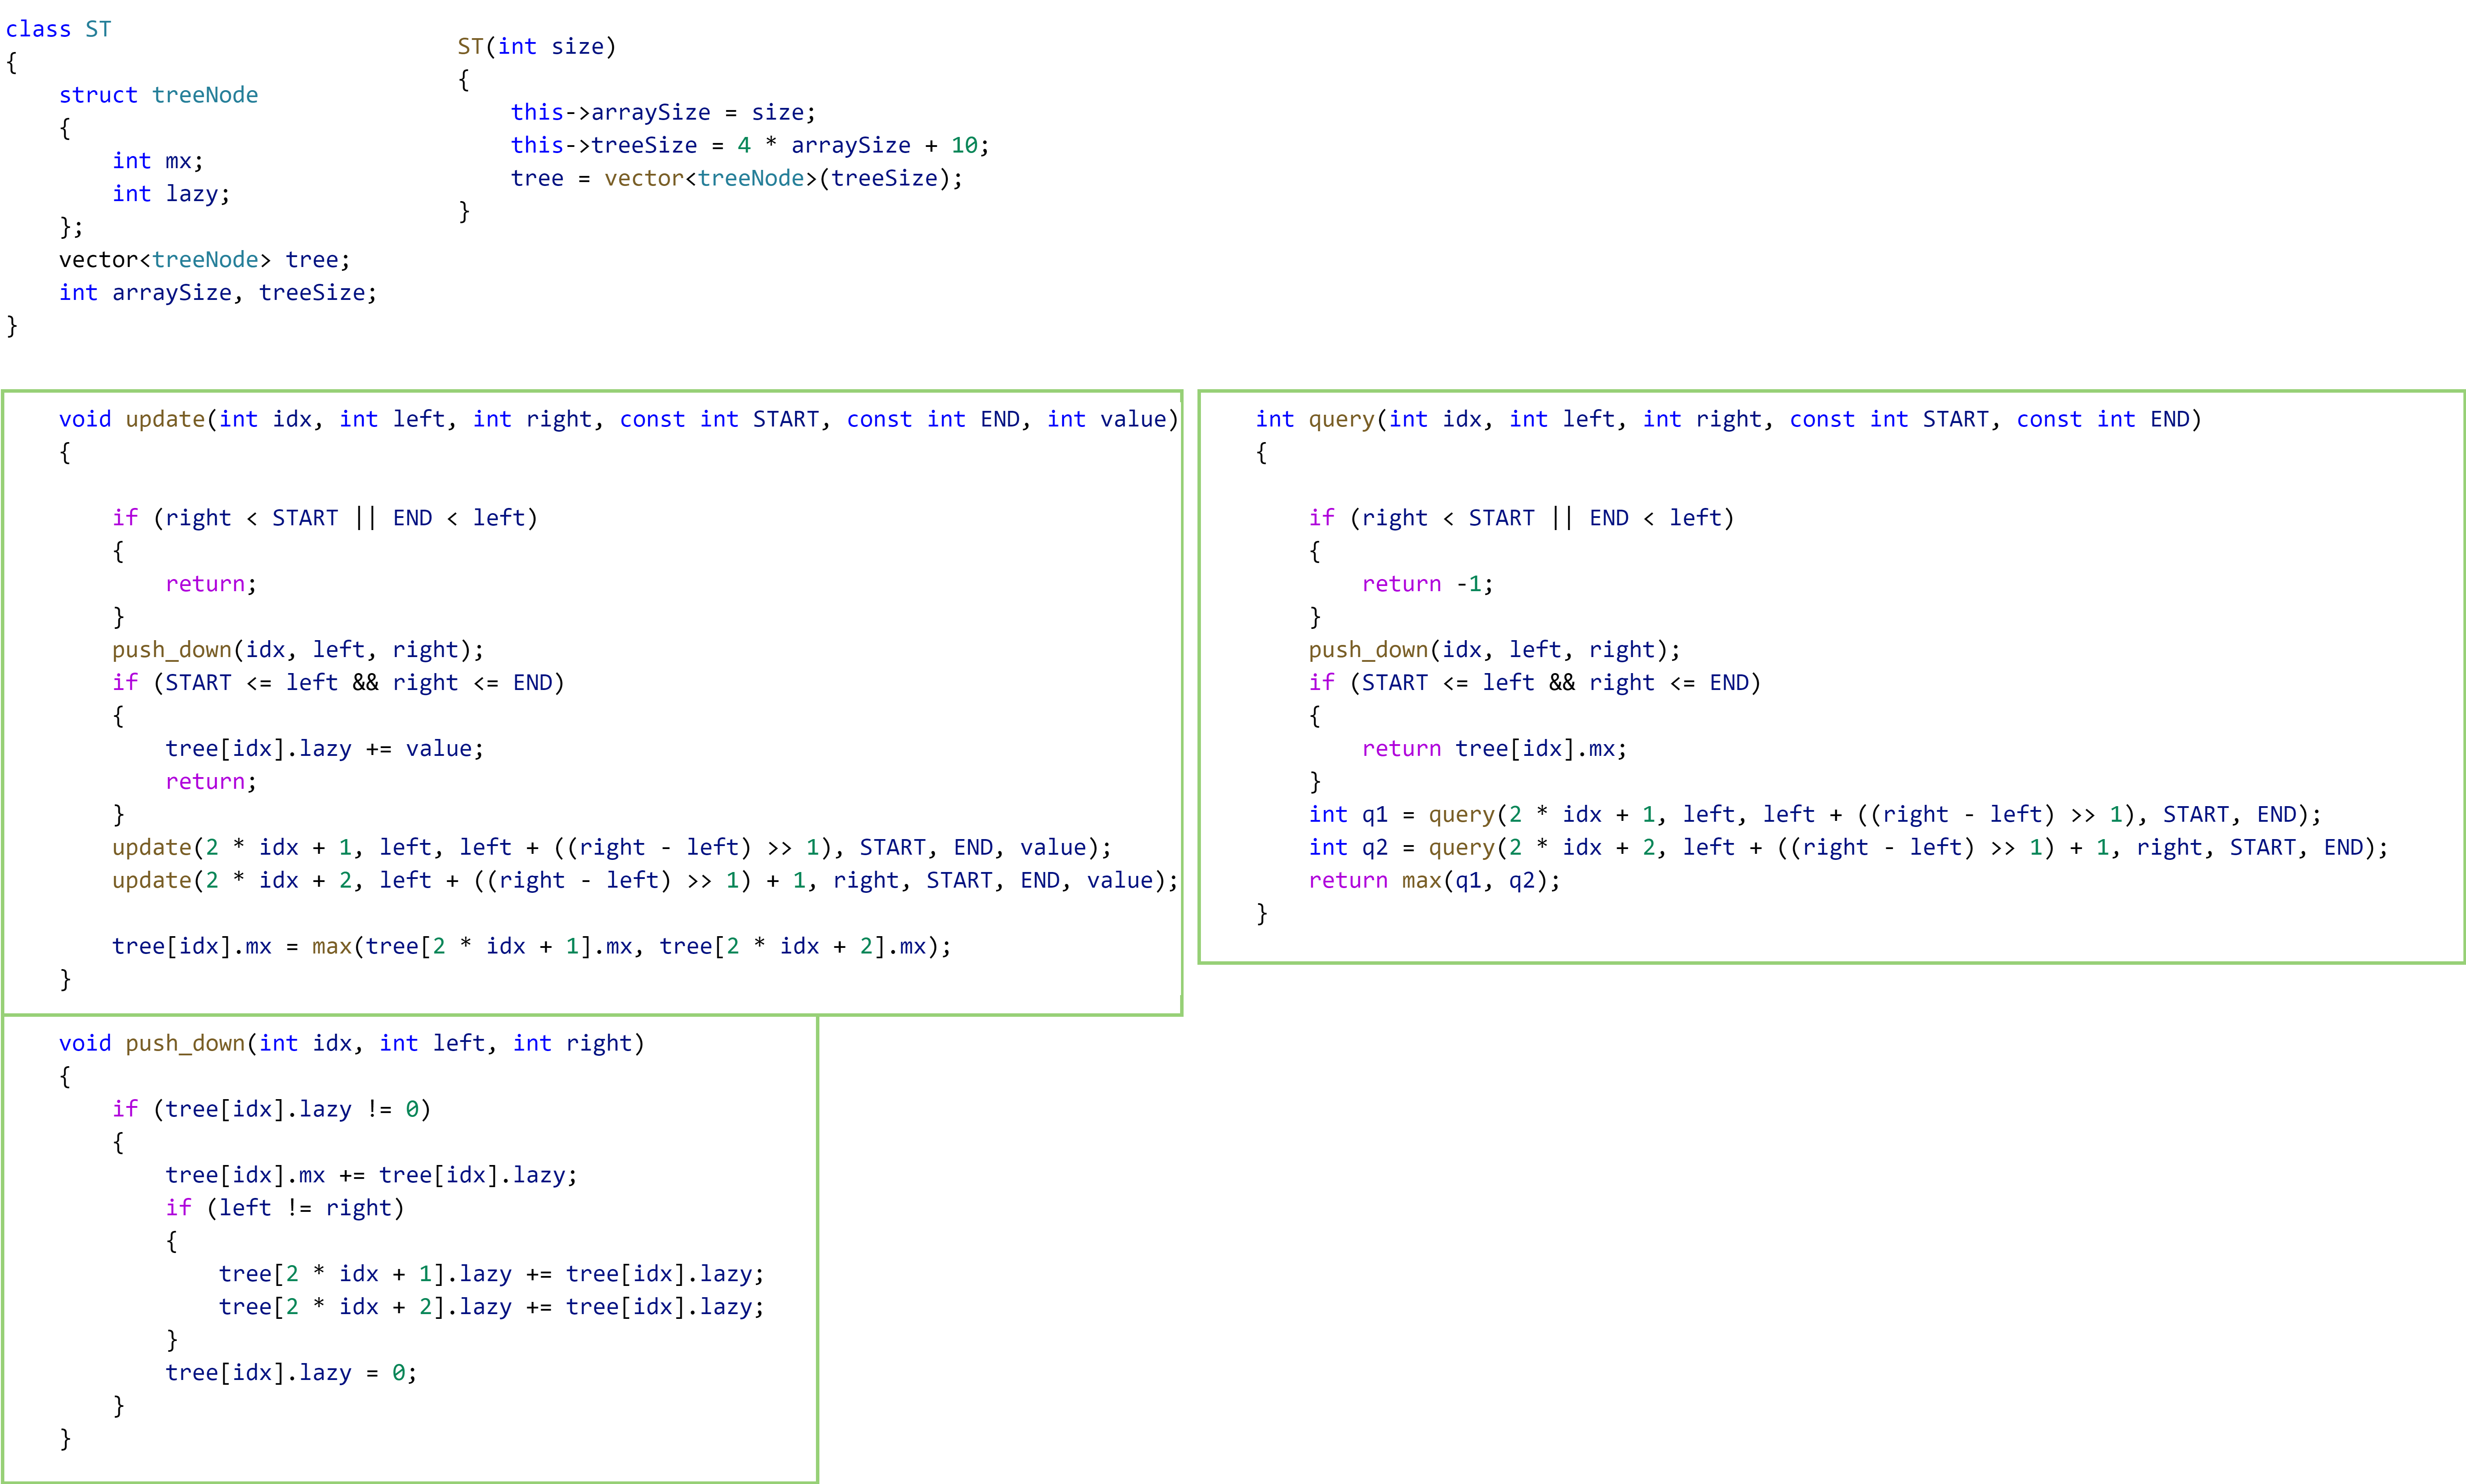
\includegraphics[width=\dimexpr\textwidth+\marginparwidth]{resources/segment-tree-2(idx).png} 
    \end{figure}


    \begin{figure}
        \caption{Segment Tree Implementation With Node}
        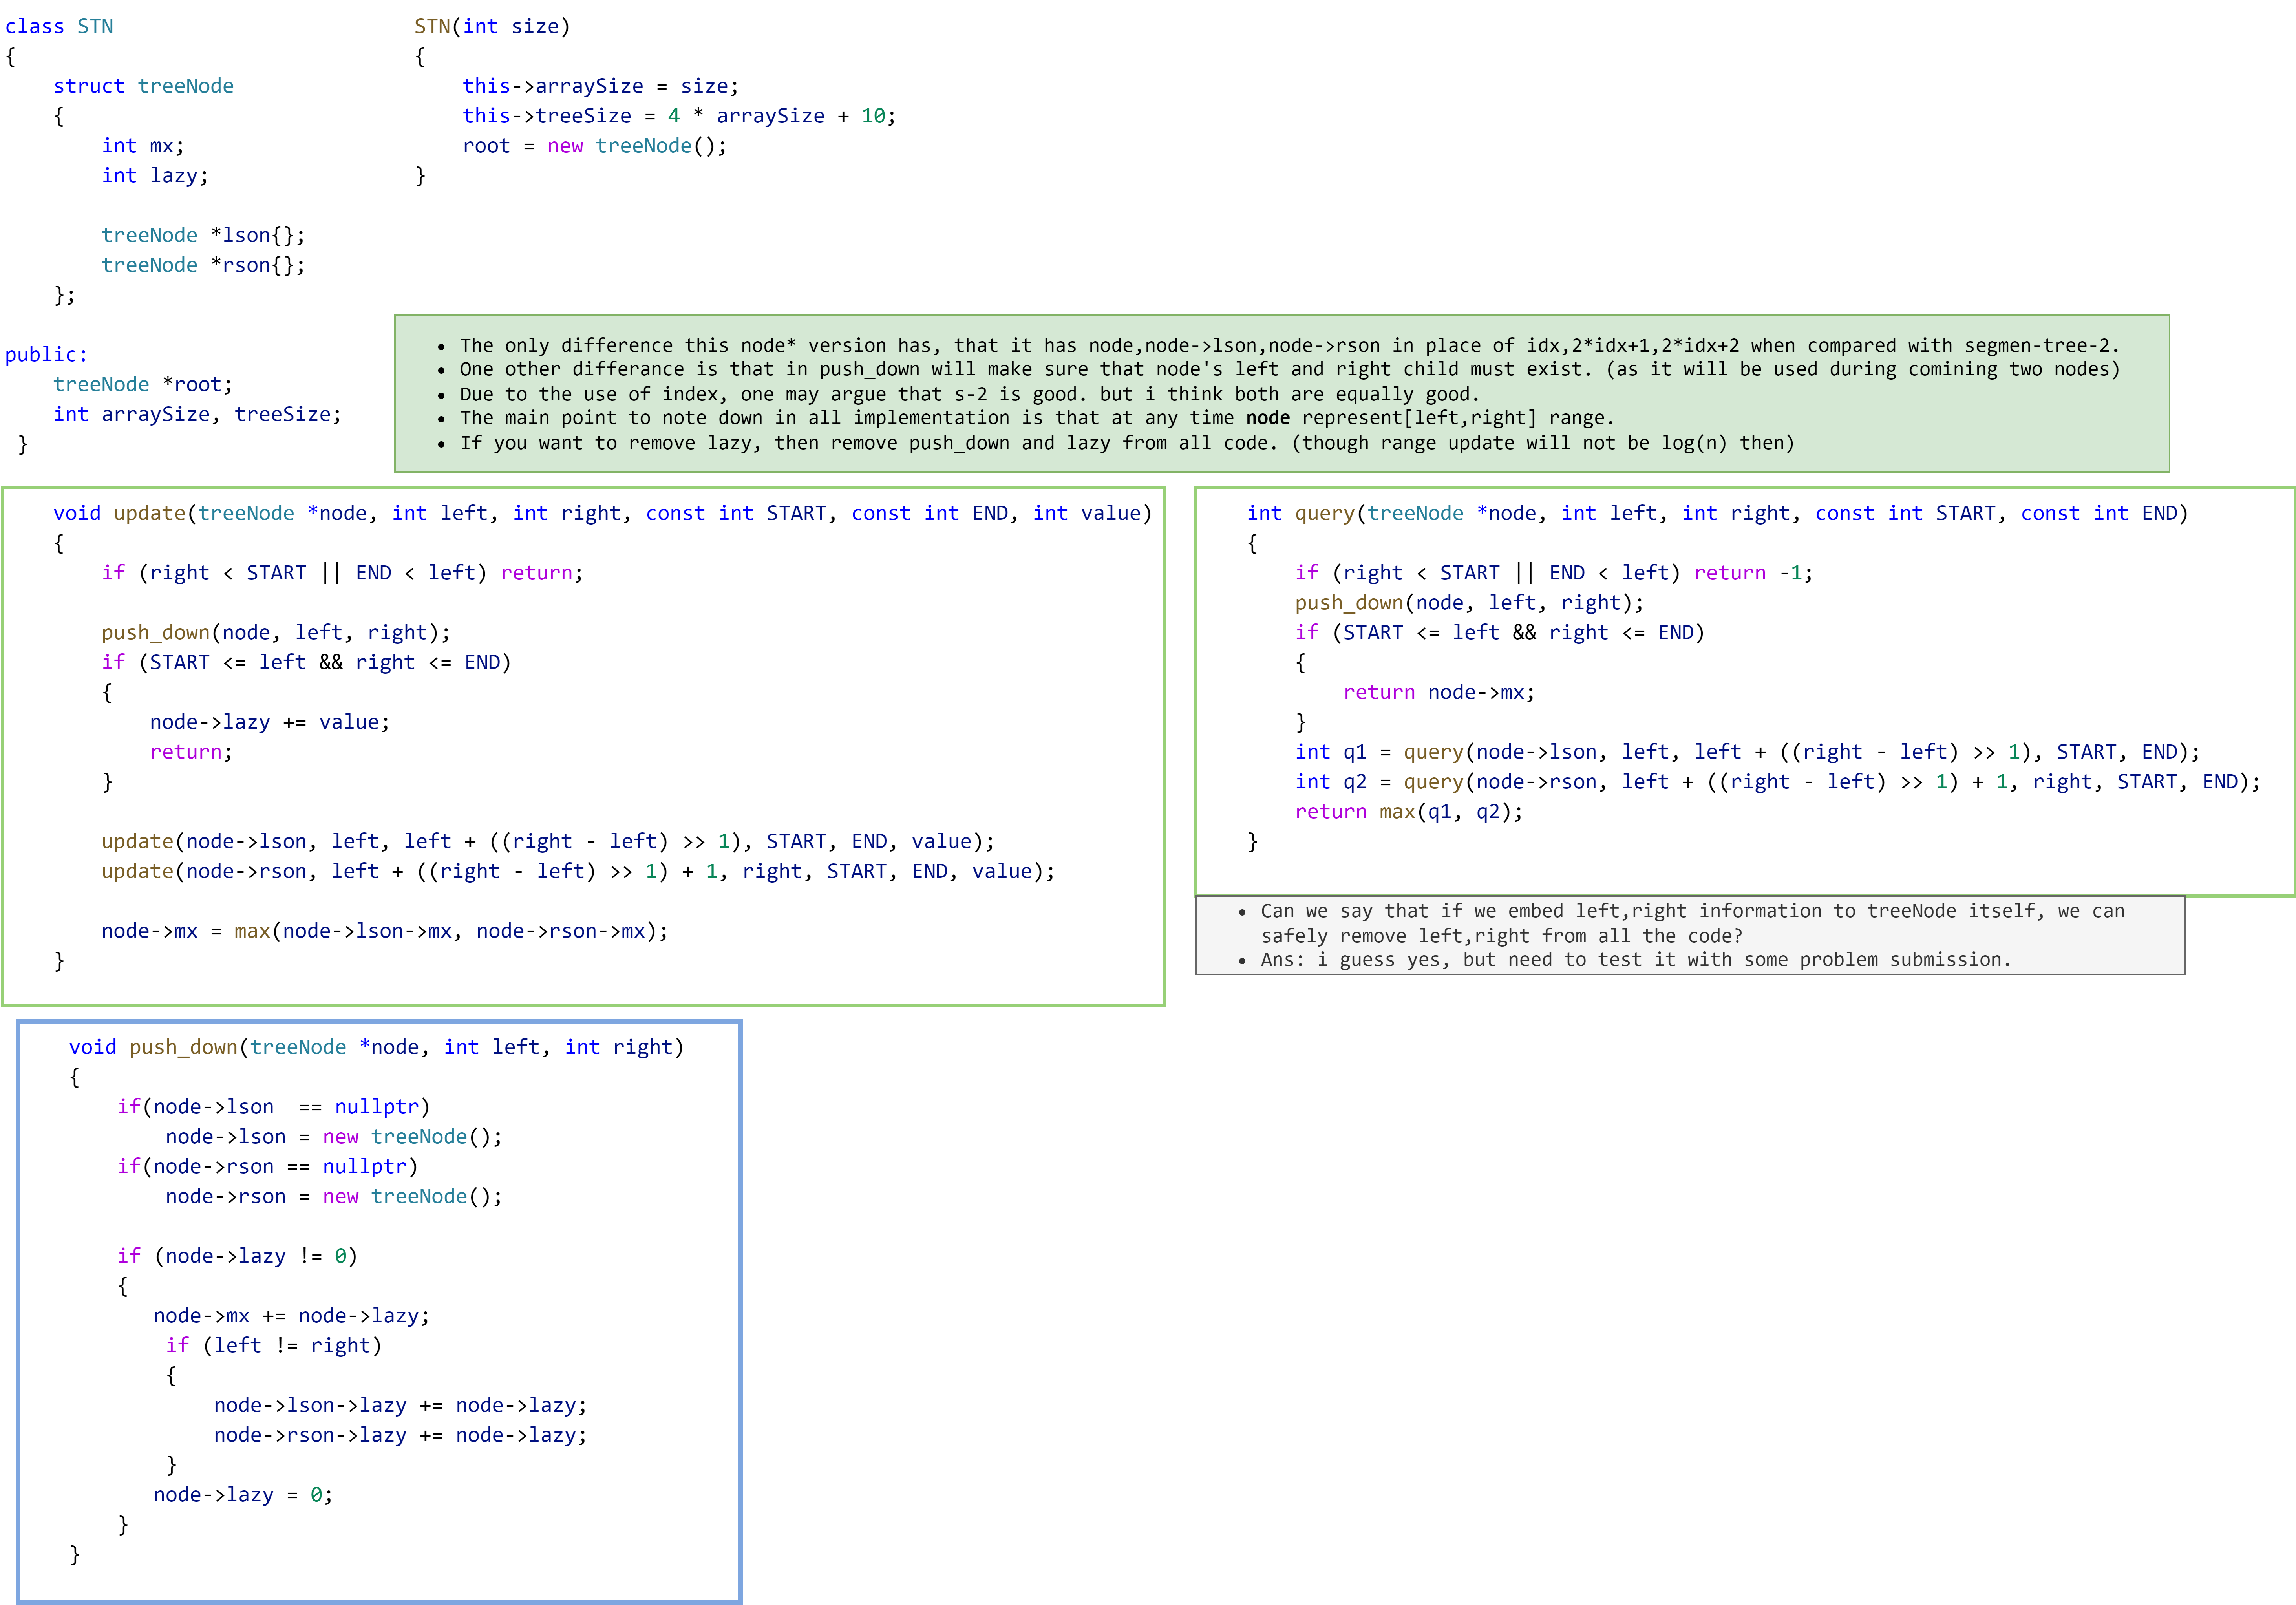
\includegraphics[width=\dimexpr\textwidth+\marginparwidth]{resources/segment-tree-3(node).png}
        
    \end{figure}

    
\end{fullwidth}

{\Large How to Debug Segment Tree?}

Array segment tree can be easiely debugged by printing all node on console. Where for each node you print following info {val,lazy,lson,rson}.
Then you check if corresponsing child nodes where called during update or query ot not.
If not$\Rightarrow$ there is a problem.
You can visualize the tree begin formed as below:


TO-DO: solve a good question , but is solvable in case of issue with above code.

fenwick tree code \href{https://cses.fi/problemset/result/6181195/}{https://cses.fi/problemset/result/6181195/}